\section{Test su immagini}
Per provare la nostra implementazione della compressione tramite DCT2, abbiamo scelto due immagini: una di Tony Pitony e una di Lena (immagine classica per l'image processing).
Per entrambe le immagini, abbiamo applicato la DCT2 con diversi valori di $f$ (la dimensione del blocco) e $d$ (il numero di coefficienti da mantenere).
Di seguito sono riportati i risultati ottenuti per ciascuna immagine, le quali sono anche disponibili in formato \texttt{.bmp} al \href{https://drive.google.com/drive/folders/1BKgunC00Pi3_k0nMBObjdeB1KHGHyaLH}{link}.
\subsection{Tony Pitony}
Per quanto riguarda l'immagine in figura \ref{fig:tony_pitony} abbiamo provato a modificare la dimensione dei blocchi $f$ e il coefficiente del taglio $d$.
I valori di $f$ che abbiamo scelto sono stati $8$, $16$, $32$, $64$ e $128$, mentre i valori di $d$ sono stati rispettivamente $4$, $8$, $16$, $32$ e $64$, ovvero la metà della dimensione del blocco.
Fare benchmark aumentando la dimensione dei blocchi può risultare interessante per questa immagine perché contiene sia aree uniformi sia dettagli ad alta frequenza, come i bordi degli occhiali e la texture della camicia.
Blocchi più grandi migliorano generalmente la compressione nelle zone lisce, ma possono introdurre artefatti più evidenti e perdita di dettaglio nelle regioni ricche di dettagli.
\begin{figure}[H]
	\centering
	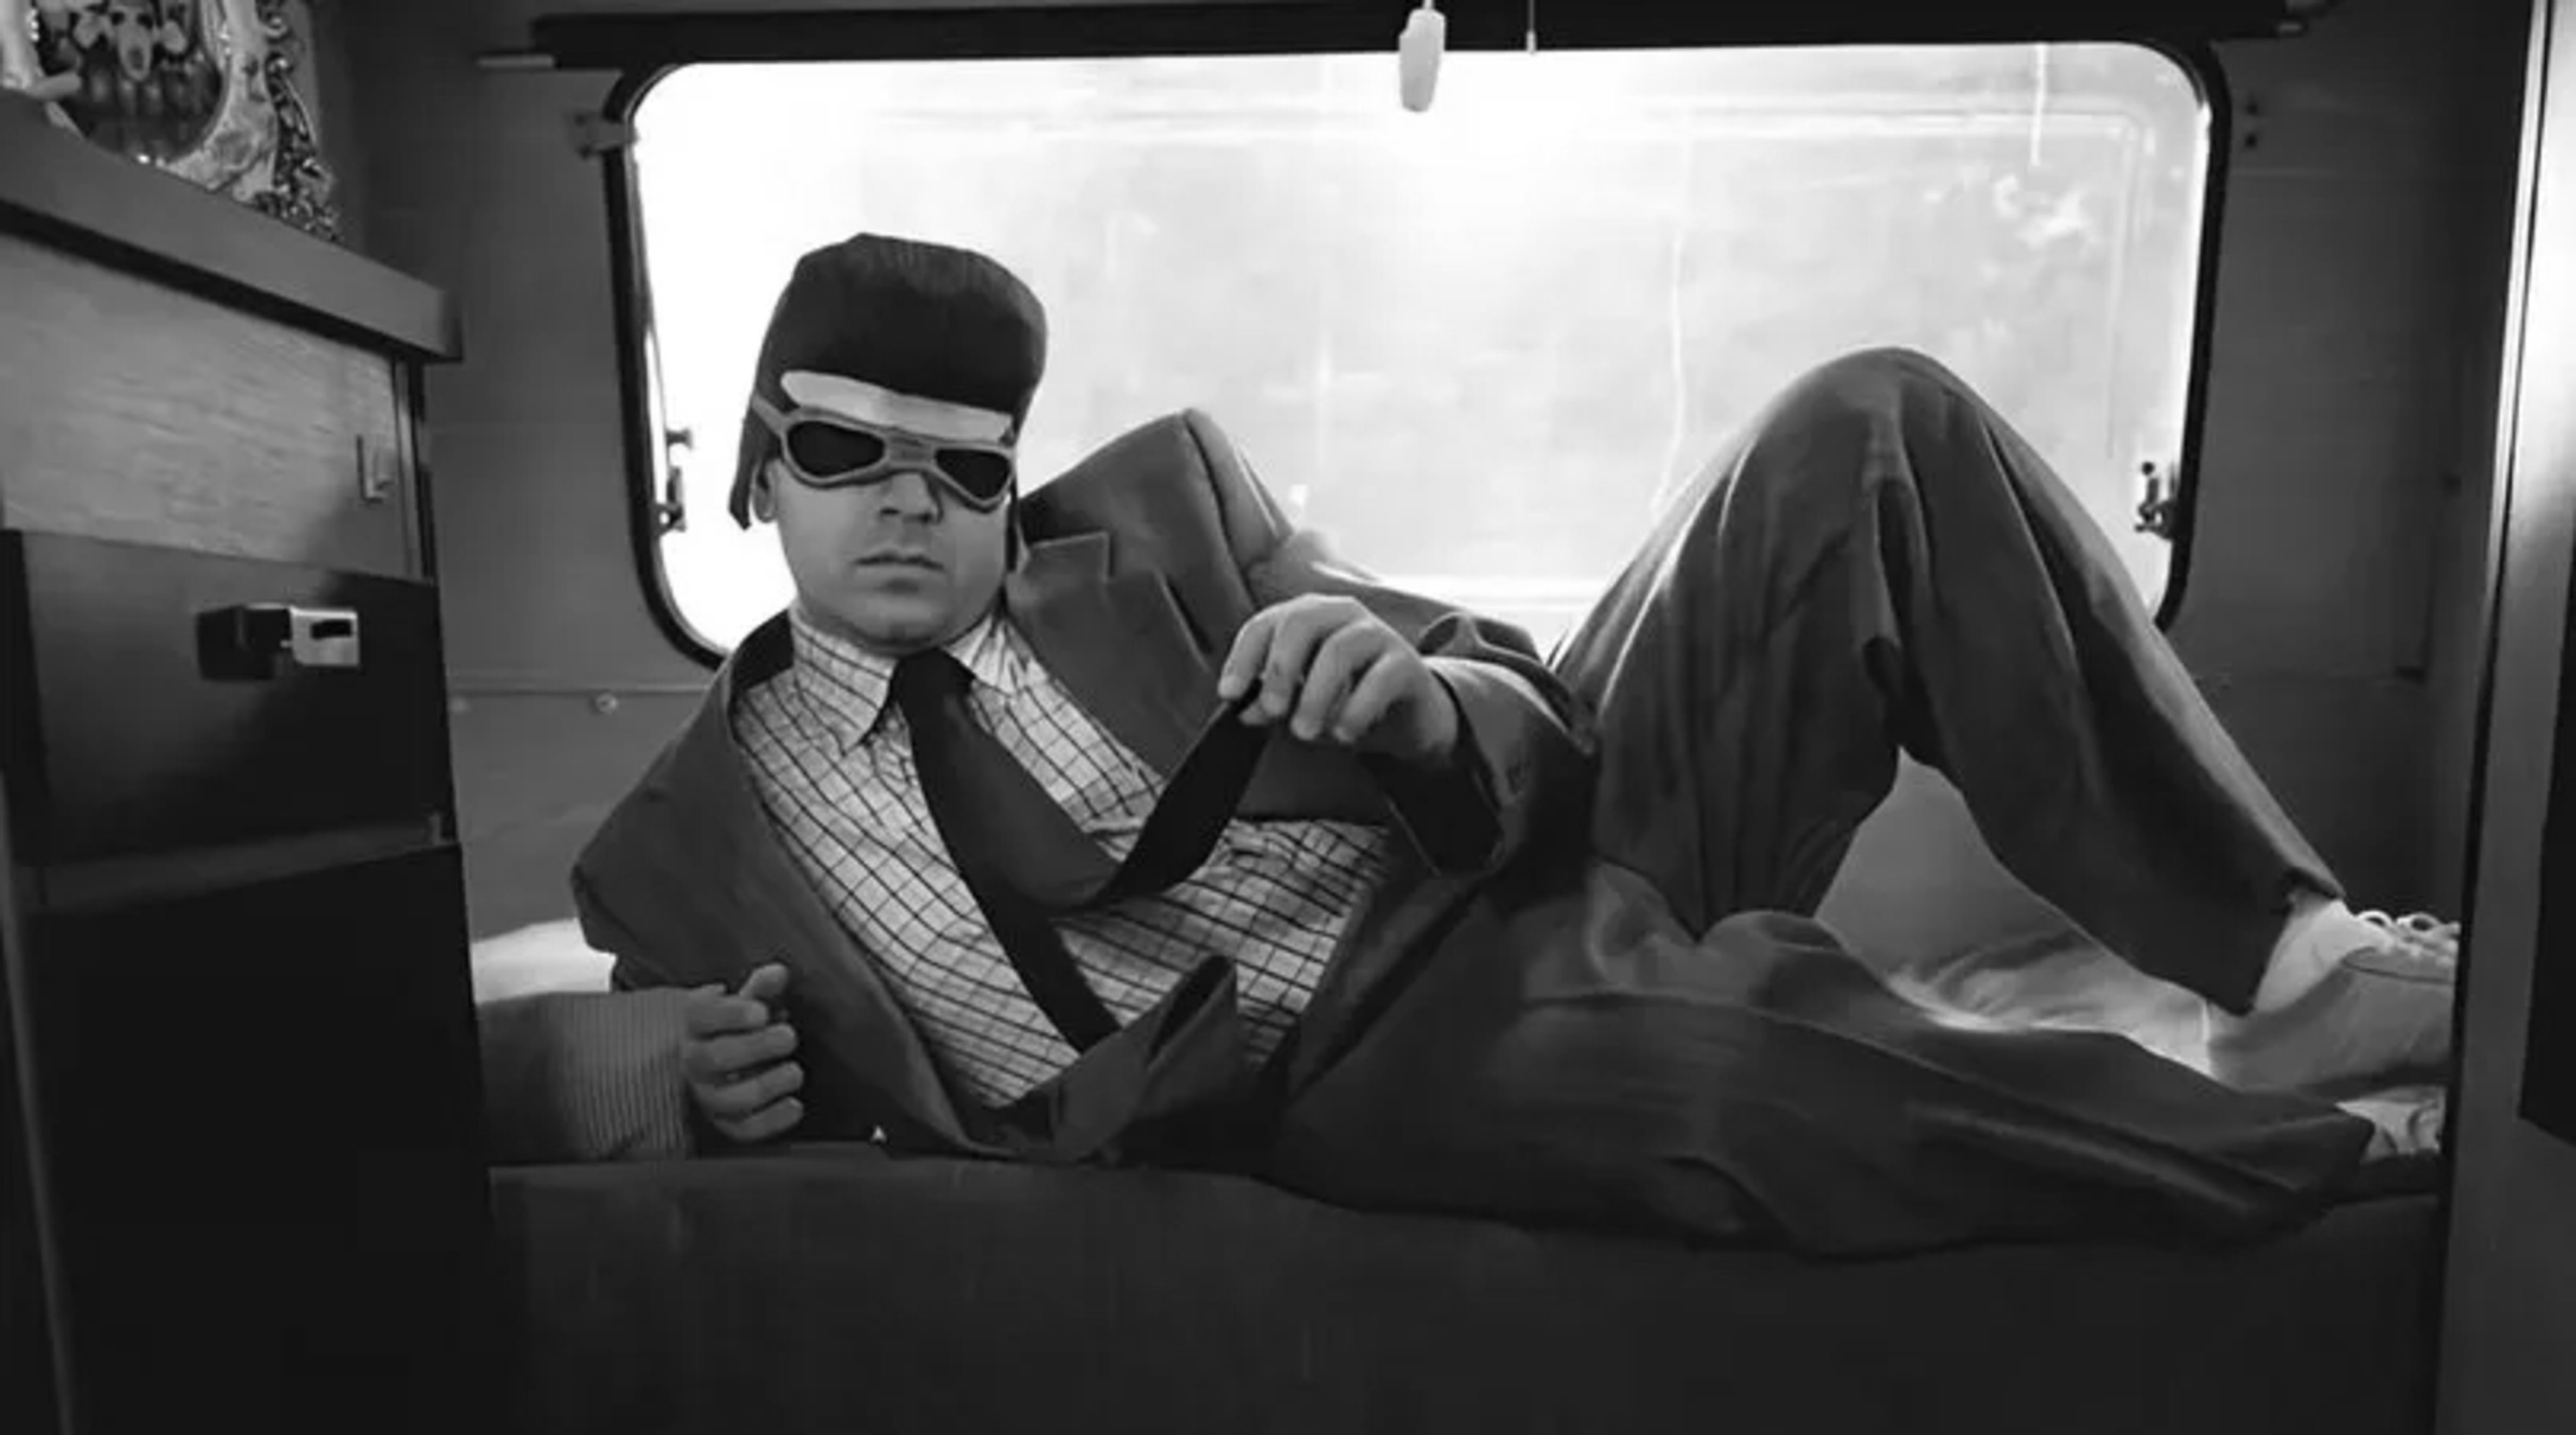
\includegraphics[width=0.8\textwidth]{figures/tonypitony.pdf}
	\caption{Immagine di Tony Pitony non compressa}
	\label{fig:tony_pitony}
\end{figure}
\begin{figure}[hbt]
	\centering
	% limit graphic size to avoid "Dimension too large" errors
	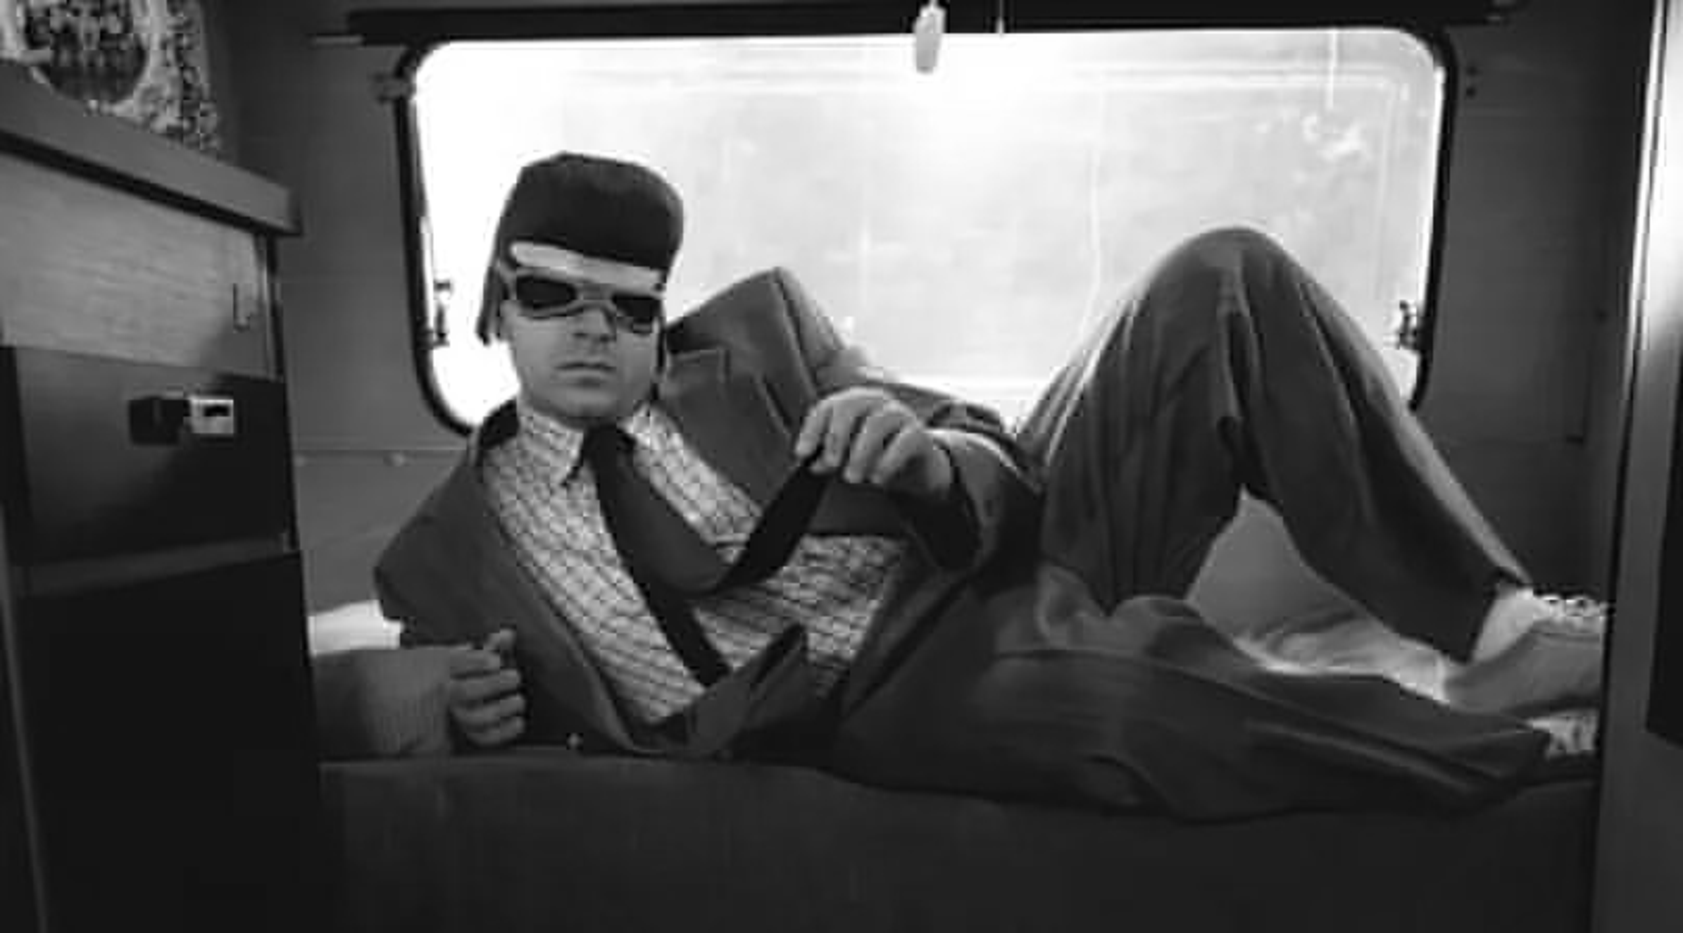
\includegraphics[width=0.8\textwidth]{figures/tonypitony_compressed_f8_d4.pdf}
	\caption{Immagine di Tony Pitony compressa con DCT2, con $f=8$ e $d=4$}
	\label{fig:tony_pitony_compressed_f8_d4}
\end{figure}
\begin{figure}[hbt]
	\centering
	% limit graphic size to avoid "Dimension too large" errors
	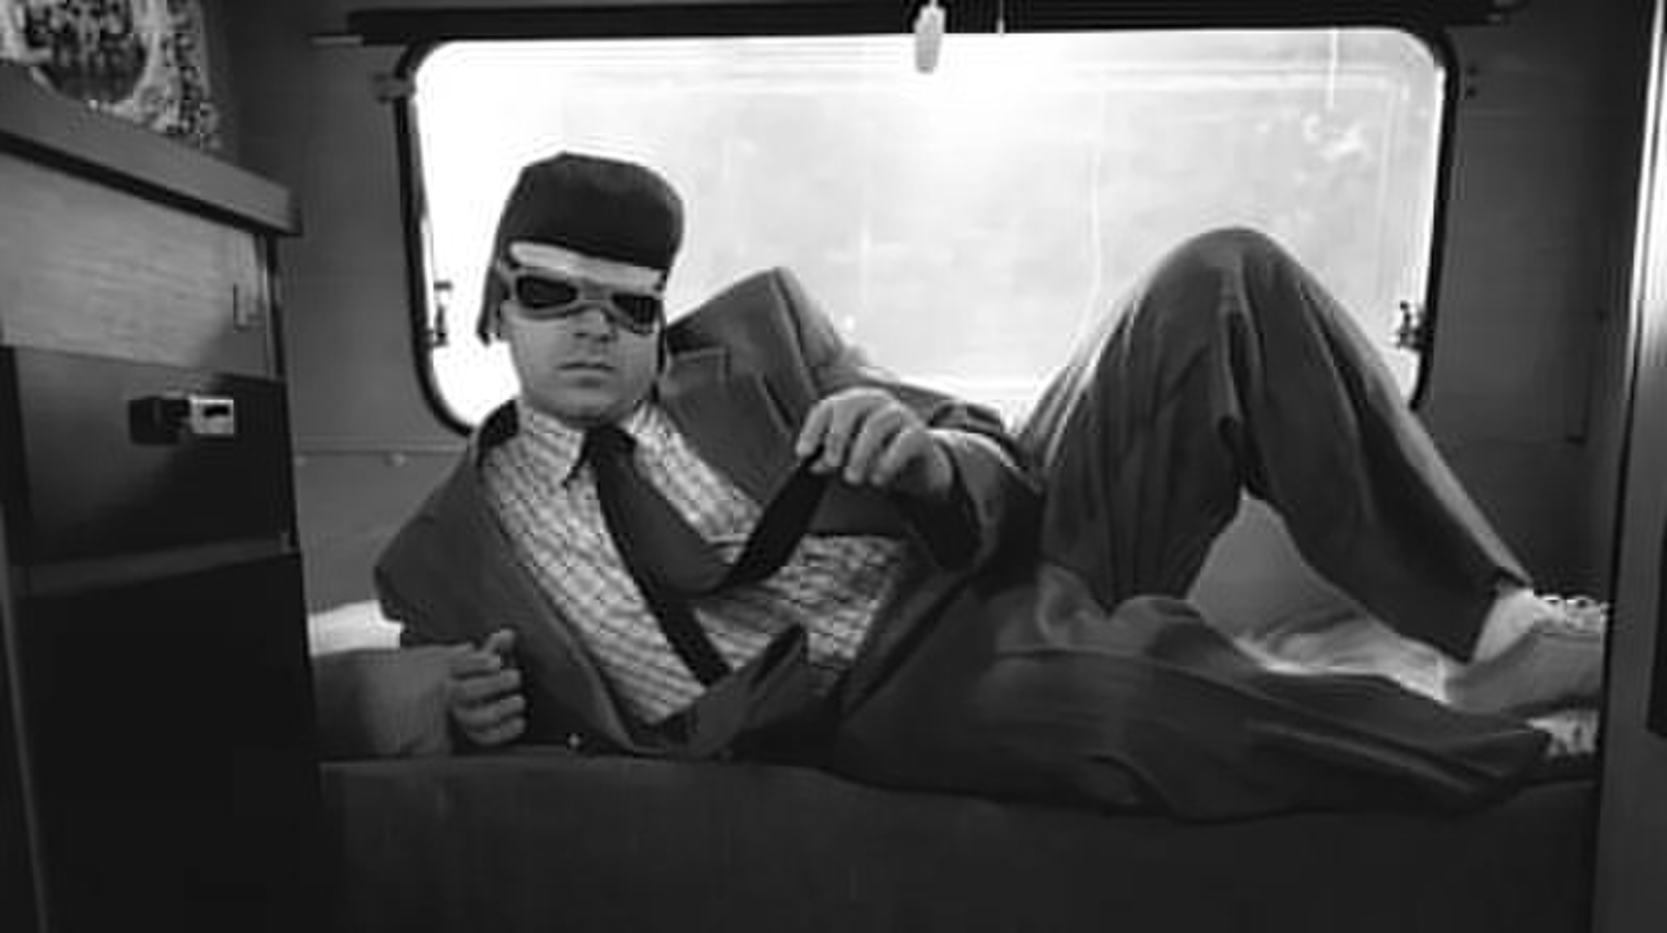
\includegraphics[width=0.8\textwidth]{figures/tonypitony_compressed_f16_d8.pdf}
	\caption{Immagine di Tony Pitony compressa con DCT2, con $f=16$ e $d=8$}
	\label{fig:tony_pitony_compressed_f16_d8}
\end{figure}
\begin{figure}[hbt]
	\centering
	% limit graphic size to avoid "Dimension too large" errors
	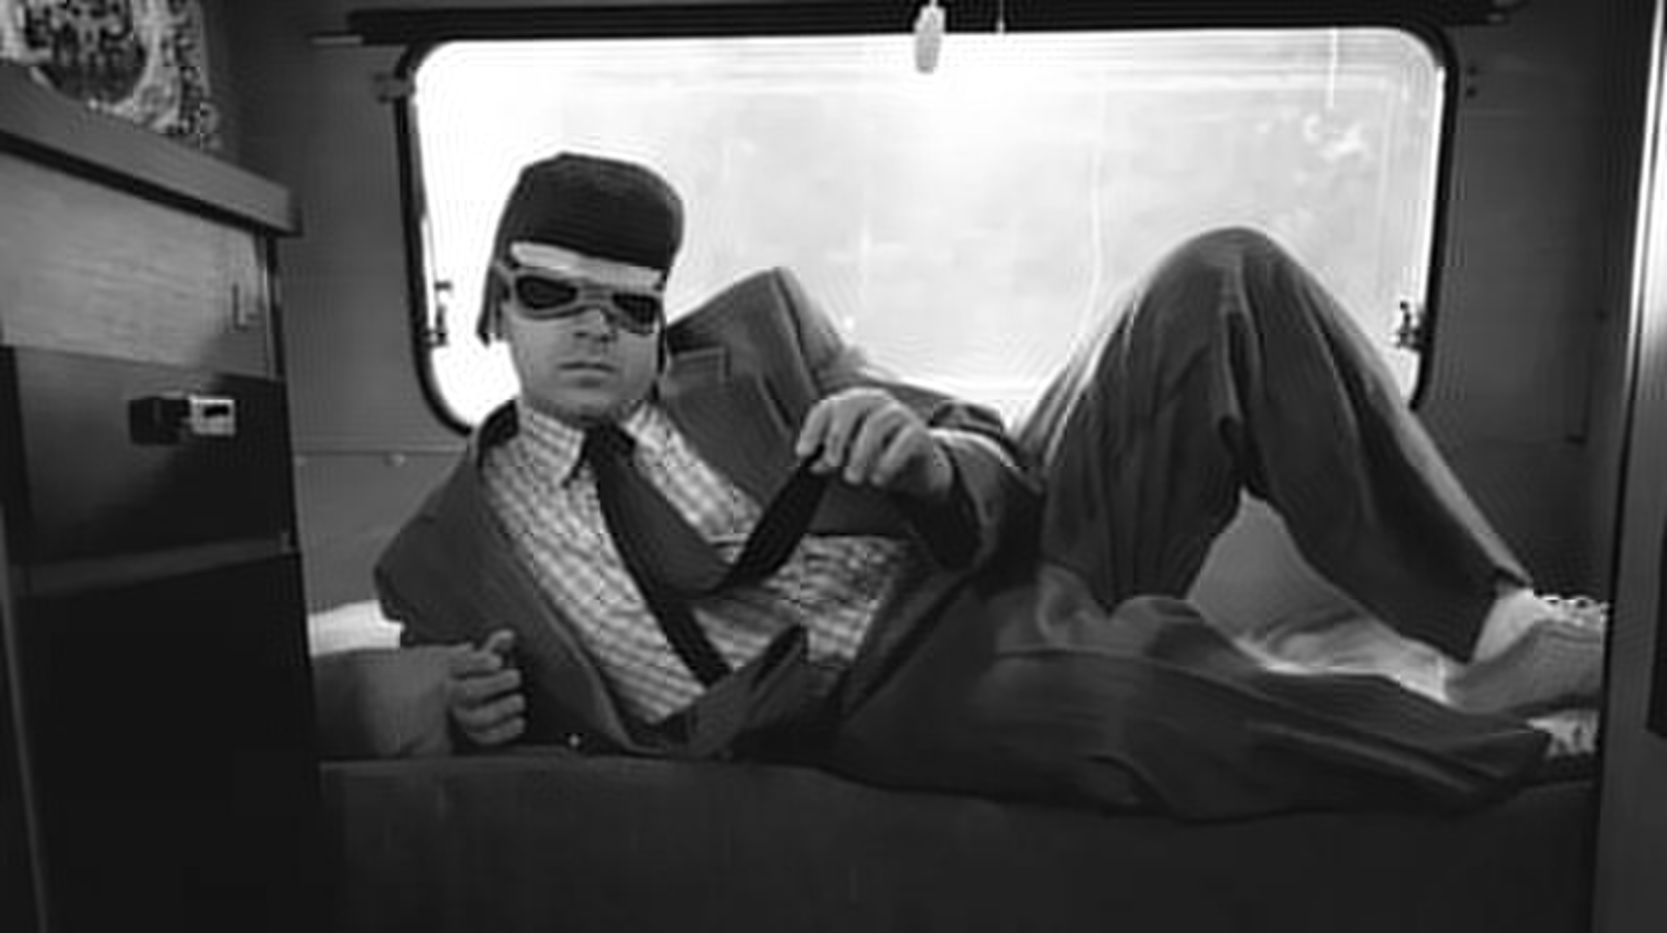
\includegraphics[width=0.8\textwidth]{figures/tonypitony_compressed_f32_d16.pdf}
	\caption{Immagine di Tony Pitony compressa con DCT2, con $f=32$ e $d=16$}
	\label{fig:tony_pitony_compressed_f32_d16}
\end{figure}

\begin{figure}[hbt]
	\centering
	% limit graphic size to avoid "Dimension too large" errors
	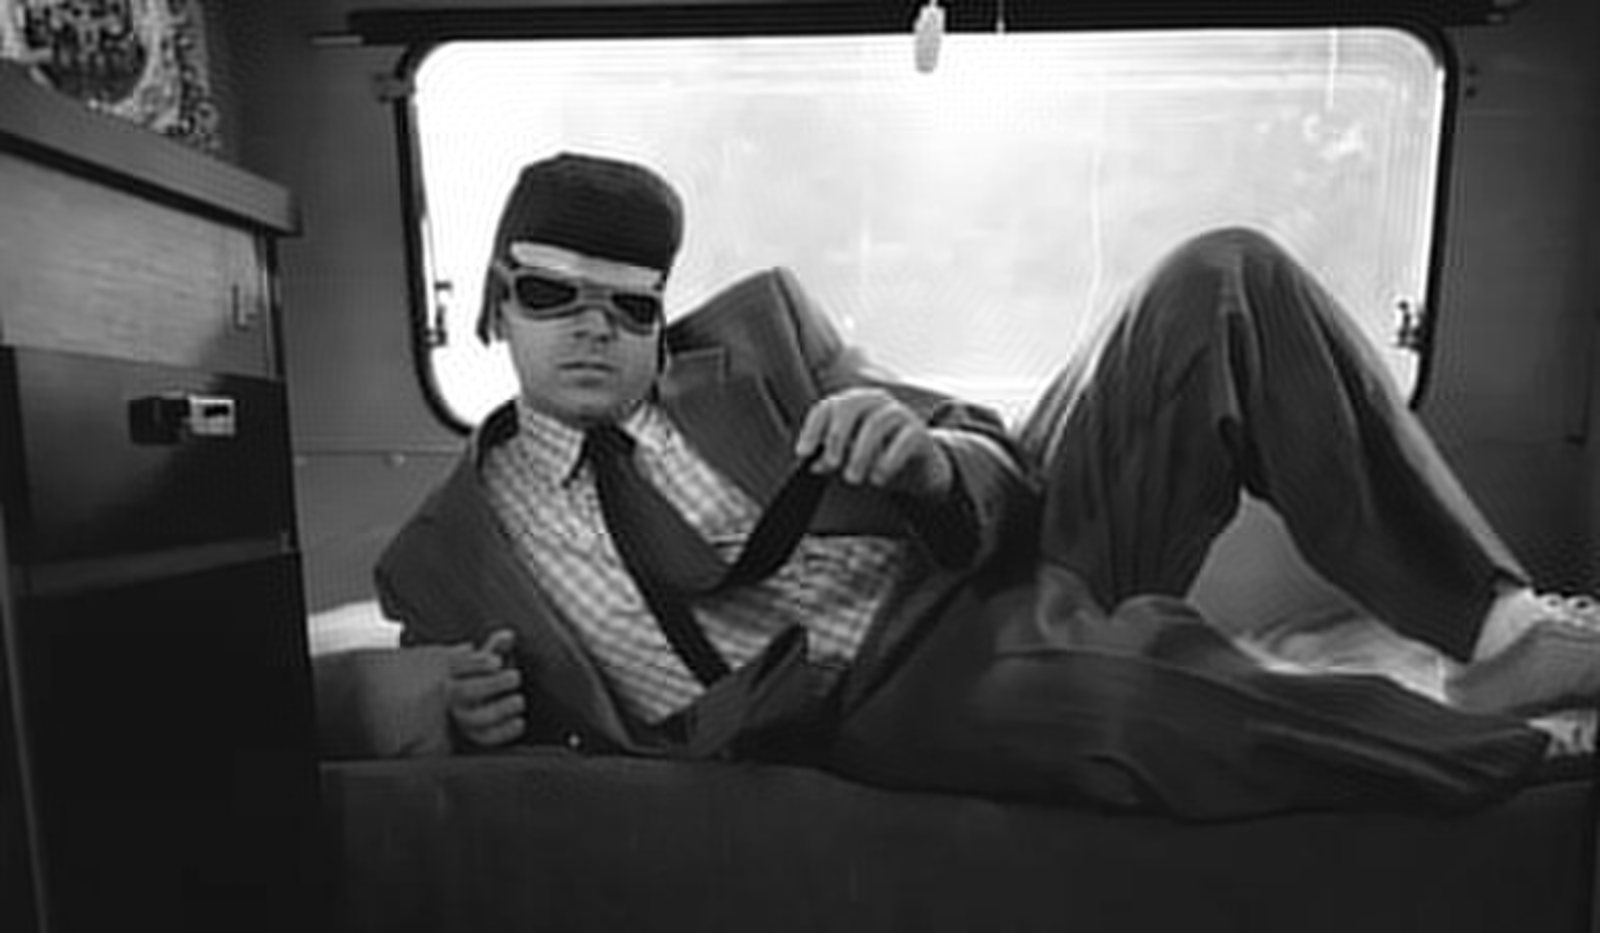
\includegraphics[width=0.8\textwidth]{figures/tonypitony_compressed_f64_d32.pdf}
	\caption{Immagine di Tony Pitony compressa con DCT2, con $f=64$ e $d=32$}
	\label{fig:tony_pitony_compressed_f64_d32}
\end{figure}
\begin{figure}[H]
	\centering
	% limit graphic size to avoid "Dimension too large" errors
	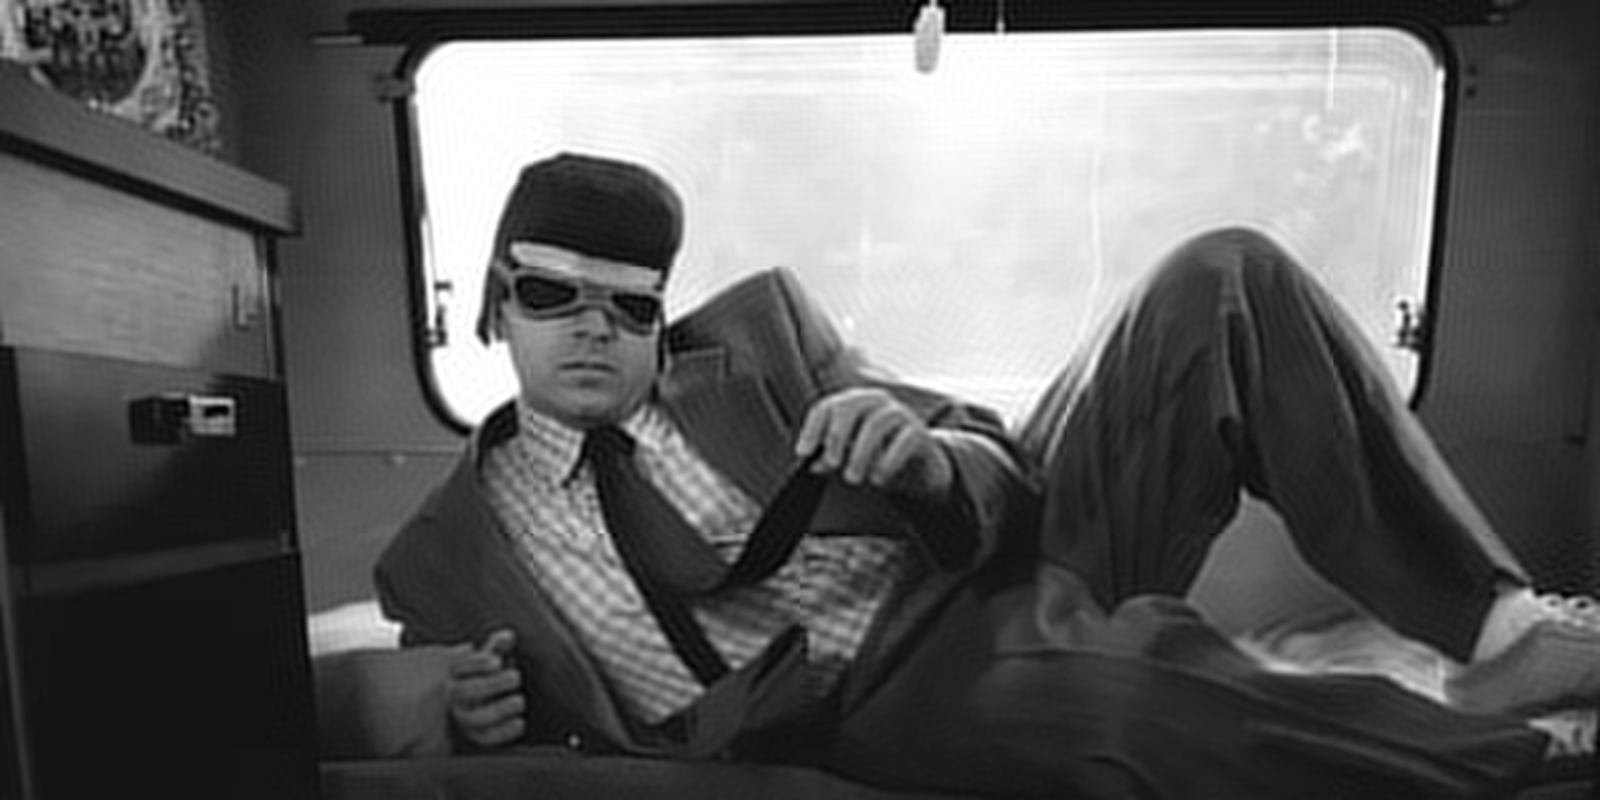
\includegraphics[width=0.8\textwidth]{figures/tonypitony_compressed_f128_d64.pdf}
	\caption{Immagine di Tony Pitony compressa con DCT2, con $f=128$ e $d=64$}
	\label{fig:tony_pitony_compressed_f128_d64}
\end{figure}
\noindent
All'aumentare della dimensione dei blocchi, possiamo vedere che la qualità dell'immagine compressa peggiora particolarmente nelle aree con molti dettagli. In particolare, si può anche notare l'introduzione di artefatti di tipo ringing nelle zone uniformi, come la finestra, che diventano più evidenti con blocchi più grandi.
Un esempio di questi artefatti è mostrato in figura \ref{fig:ringing}, dove si possono vedere delle bande scure e chiare intorno ai bordi, tipiche del fenomeno di ringing.
L'effetto sulle nostre immagini è evidenziato in figura \ref{fig:tony_pitony_ringing}, dove si possono notare le bande scure attorno alla gamba e ai bordi della finestra.
\begin{figure}[H]
	\centering
	% limit graphic size to avoid "Dimension too large" errors
	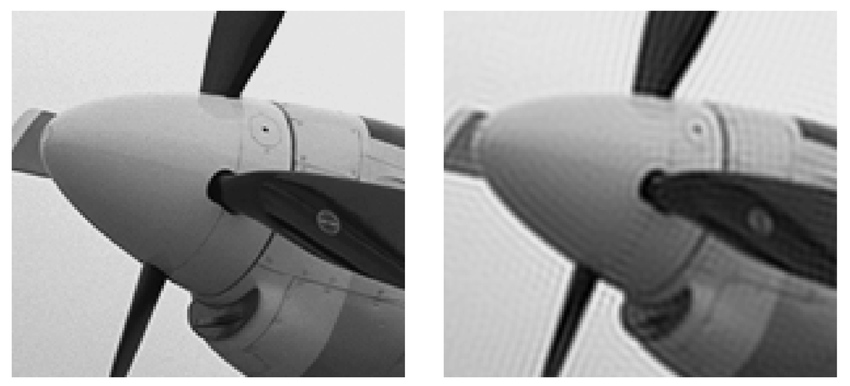
\includegraphics[width=0.8\textwidth]{figures/ringing.png}
	\caption{Artefatti di tipo ringing}
	\label{fig:ringing}
\end{figure}
\begin{figure}[H]
	\centering
	% limit graphic size to avoid "Dimension too large" errors
	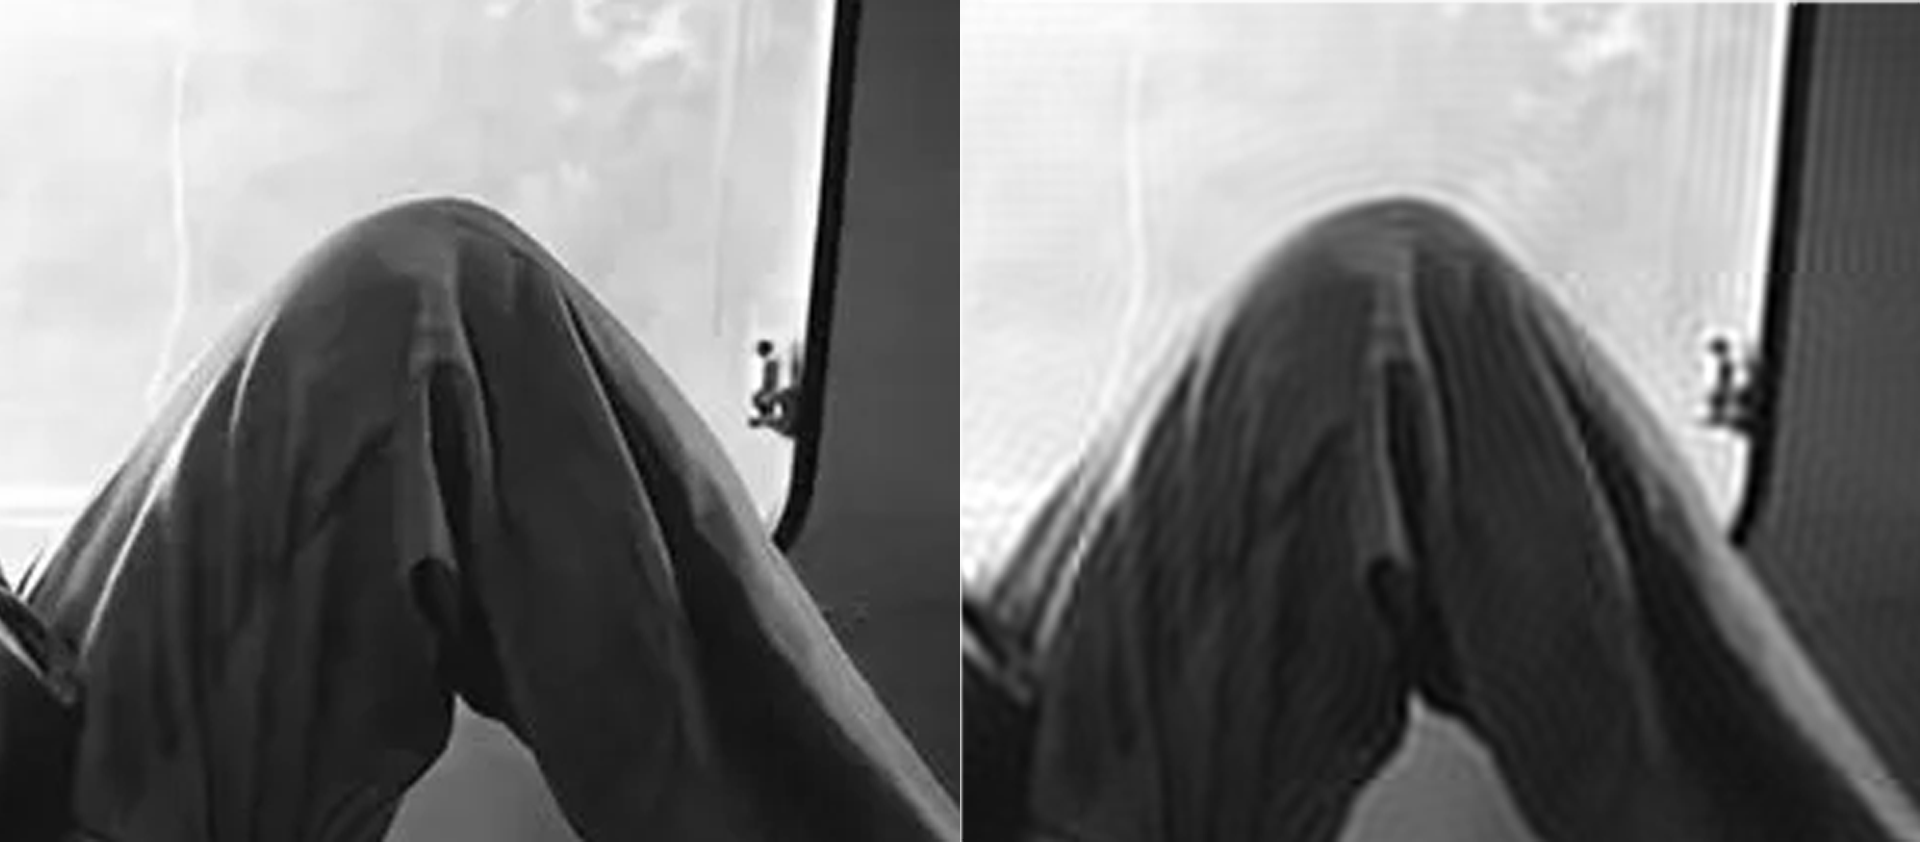
\includegraphics[width=0.8\textwidth]{figures/ringingTonyPitony.png}
	\caption{Zoom sull'immagine di Tony Pitony compressa con DCT2, con $f=128$ e $d=64$, evidenziando gli artefatti di tipo ringing}
	\label{fig:tony_pitony_ringing}
\end{figure}
\subsection{Lena}
Per quanto riguarda l'immagine in figura \ref{fig:lena} abbiamo provato a mantenere fissa la dimensione dei blocchi $f$ a $8$ e a modificare il coefficiente del taglio $d$ con i valori $12$, $8$, $4$, $2$ e $0$.
In particolare, con $d=0$ abbiamo eliminato tutti i coefficienti, ottenendo così un'immagine completamente nera.
Si può osservare che, come ci si aspetta, all'aumentare del numero di coefficienti mantenuti, la qualità dell'immagine compressa migliora, con una maggiore fedeltà all'immagine originale.
In particolare, con $d=12$ e $d=8$ l'immagine compressa è molto simile all'originale, mentre con $d=4$ si notano perdite di dettagli e si manifesta il tipico effetto di jpeg dove sono ben visibili i blocchi di dimensione $8\times8$.
\clearpage
\begin{multicols}{2}
\begin{figure}[H]
	\centering
	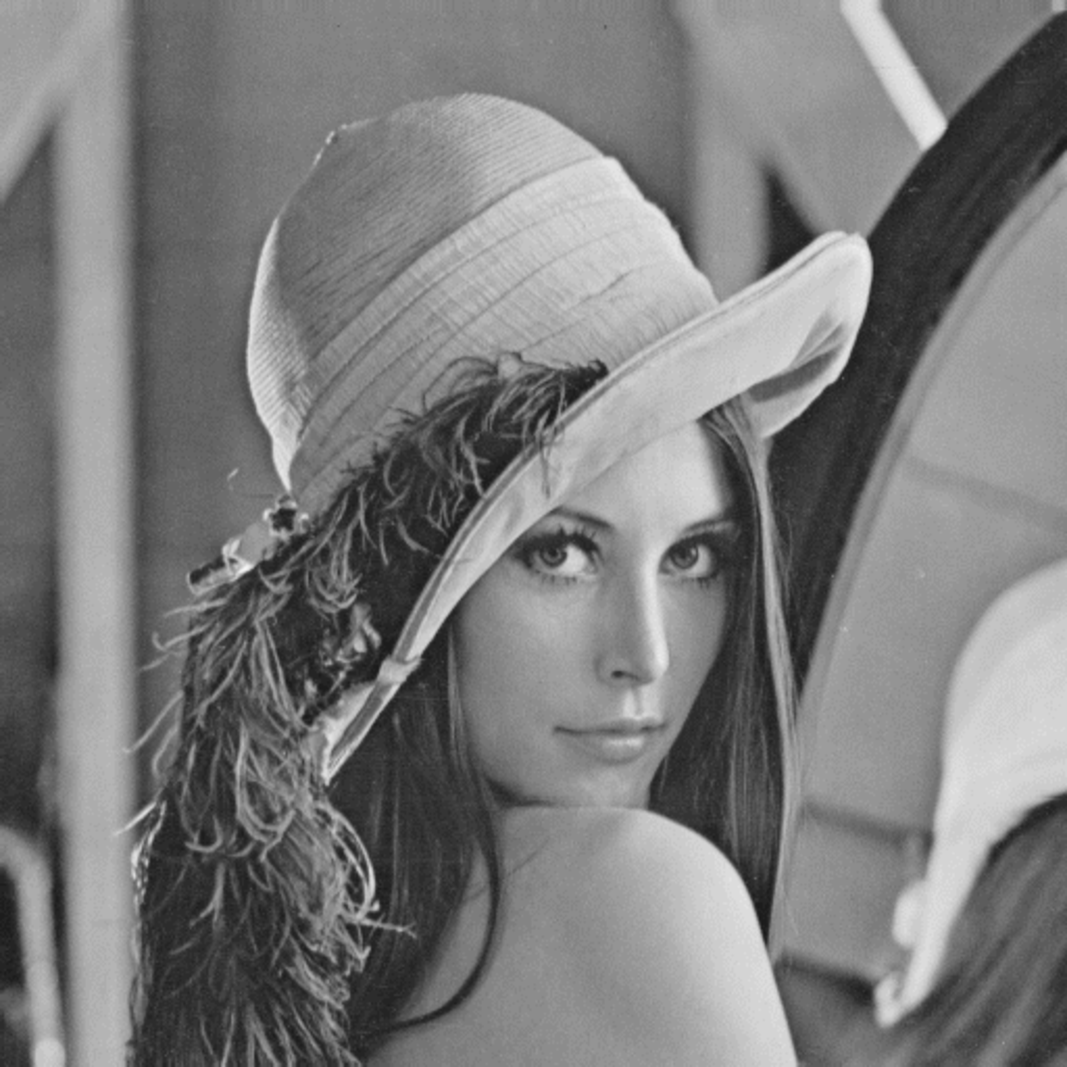
\includegraphics[width=0.49\textwidth]{figures/lena.pdf}
	\caption{Immagine di Lena non compressa}
	\label{fig:lena}
\end{figure}
\columnbreak
\begin{figure}[H]
	\centering
	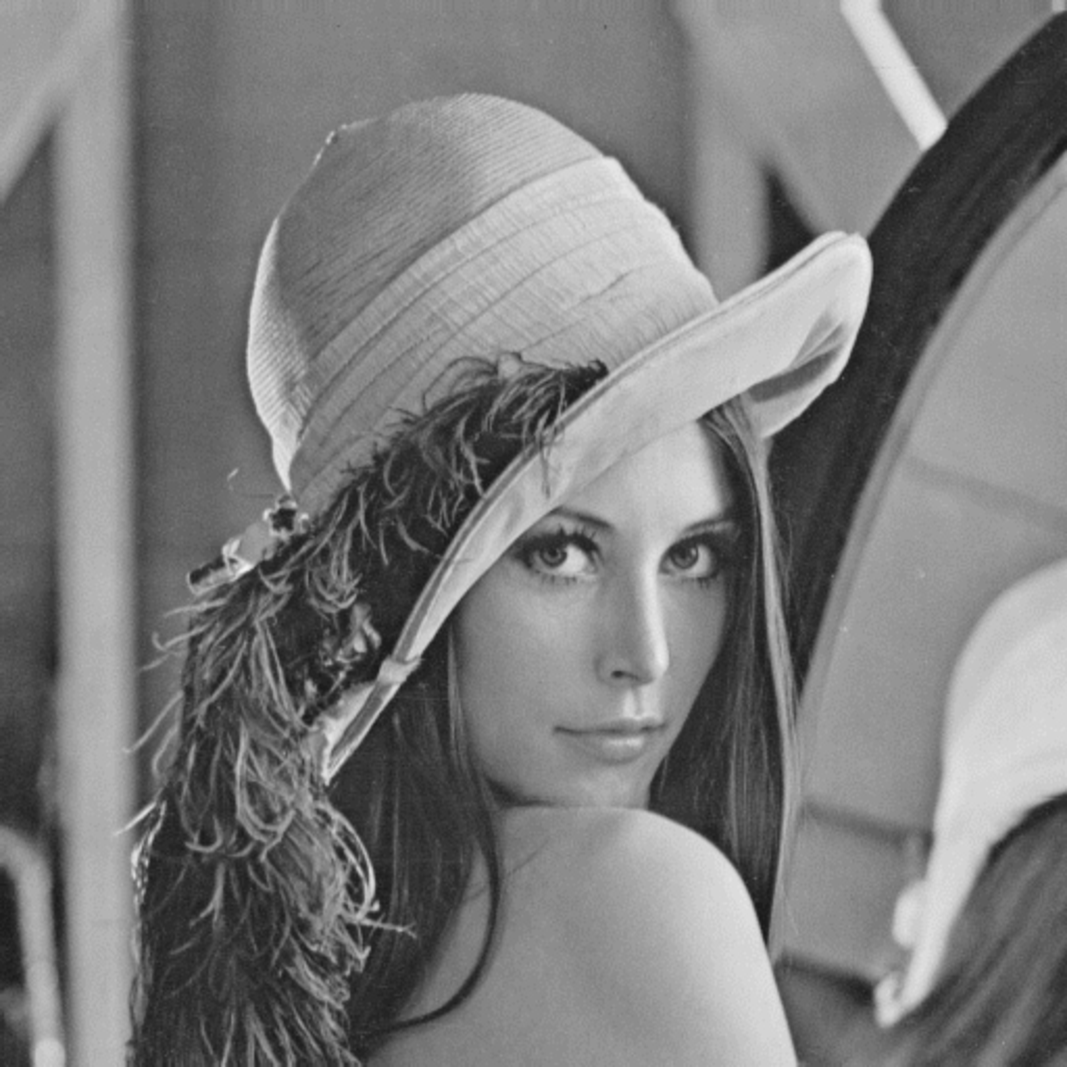
\includegraphics[width=0.49\textwidth]{figures/lena_compressed_f8_d12.pdf}
	\caption{Immagine di Lena compressa con DCT2, con $f=8$ e $d=12$}
	\label{fig:lena_compressed_f8_d12}
\end{figure}
\end{multicols}
\begin{multicols}{2}
\begin{figure}[H]
	\centering
	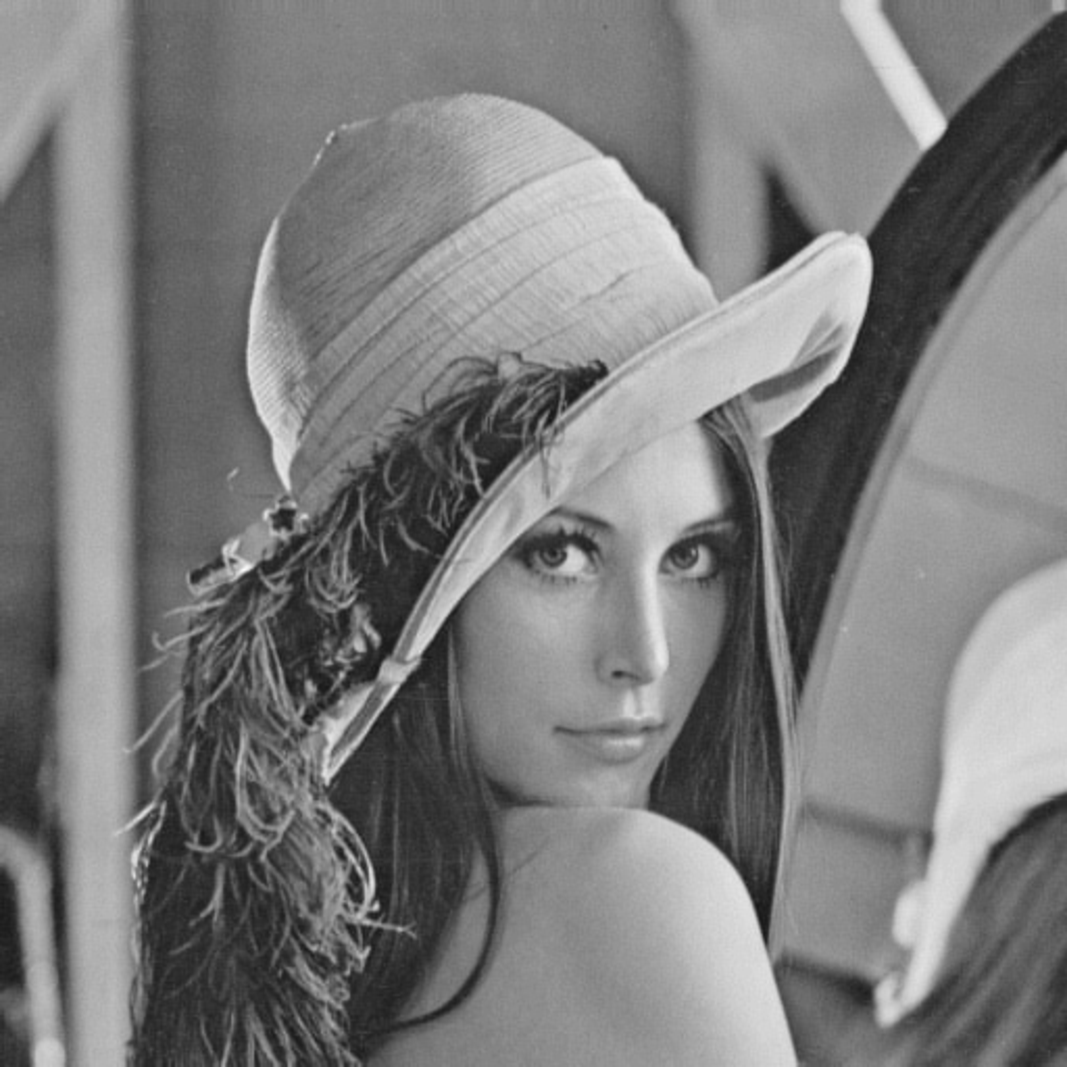
\includegraphics[width=0.5\textwidth]{figures/lena_compressed_f8_d8.pdf}
	\caption{Immagine di Lena compressa con DCT2, con $f=8$ e $d=8$}
	\label{fig:lena_compressed_f8_d8}
\end{figure}
\columnbreak
\begin{figure}[H]
	\centering
	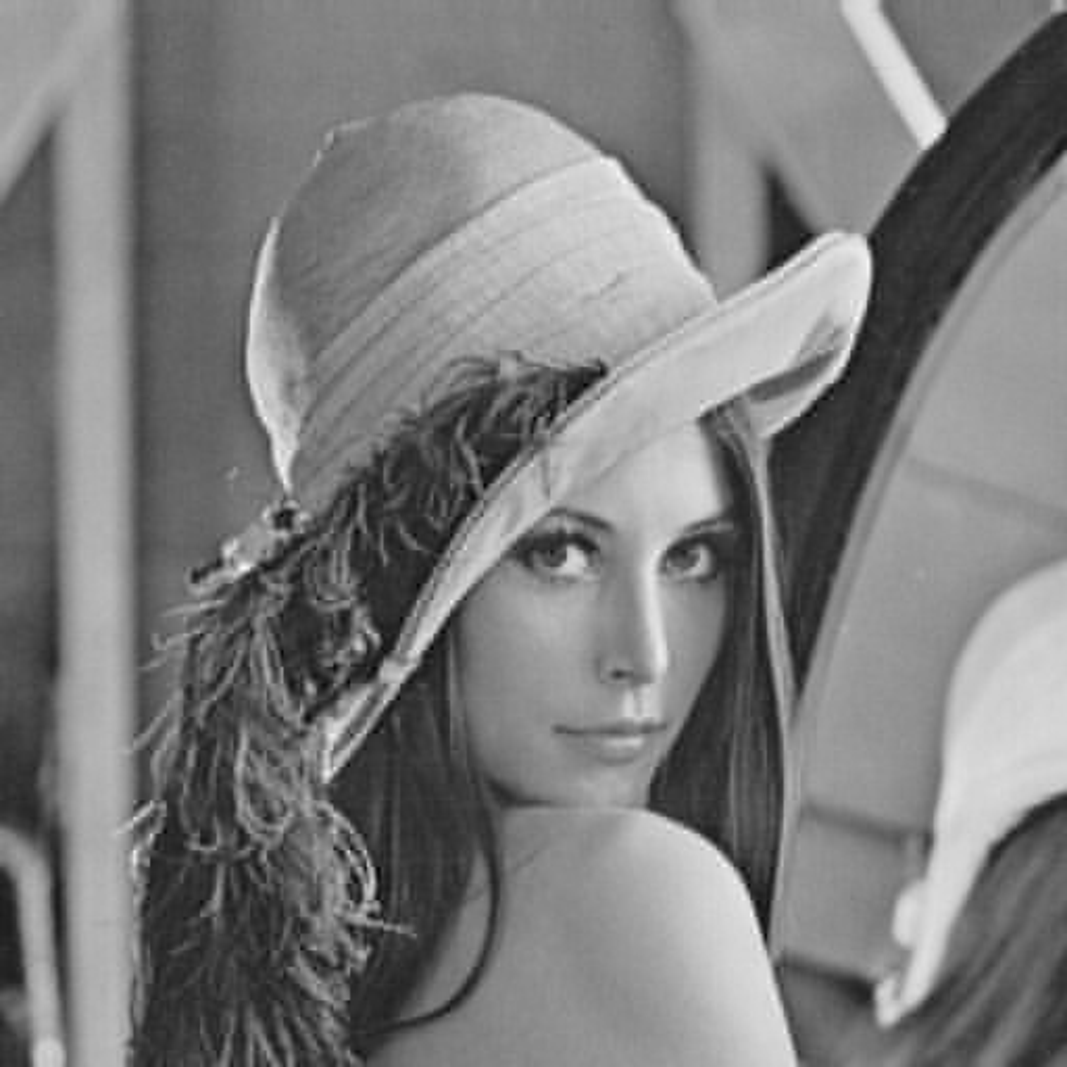
\includegraphics[width=0.5\textwidth]{figures/lena_compressed_f8_d4.pdf}
	\caption{Immagine di Lena compressa con DCT2, con $f=8$ e $d=4$}
	\label{fig:lena_compressed_f8_d4}
\end{figure}
\end{multicols}
\clearpage

\begin{multicols}{2}
	
\begin{figure}[H]
	\centering
	
\includegraphics[width=0.5\textwidth]{figures/lena_compressed_f8_d2.pdf}
	\caption{Immagine di Lena compressa con DCT2, con $f=8$ e $d=2$}
	\label{fig:lena_compressed_f8_d2}
\end{figure}
\columnbreak
\begin{figure}[H]
	\centering
	
\includegraphics[width=0.5\textwidth]{figures/lena_compressed_f8_d0.pdf}
	\caption{Immagine di Lena compressa con DCT2, con $f=8$ e $d=0$}
	\label{fig:lena_compressed_f8_d0}
\end{figure}
\end{multicols}
